\documentclass[24pt]{article}
\usepackage{graphicx}
\usepackage[margin=0.6in]{geometry}
\usepackage{xcolor}
\usepackage{amssymb}
\usepackage{subcaption}
\usepackage{amsmath}
\DeclareRobustCommand{\rchi}{{\mathpalette\irchi\relax}}
\newcommand{\irchi}[2]{\raisebox{\depth}{$#1\chi$}} % inner command, used by \rchi
\usepackage{pgfplots}
\usepackage{tikz}
\pgfplotsset{width=10cm,compat=1.9}
\usepgfplotslibrary{external}
\tikzexternalize
\definecolor{green}{rgb}{0.1,0.5,0.1}
\definecolor{codegray}{rgb}{0.5,0.5,0.5}
\definecolor{codepurple}{rgb}{0.58,0,0.82}
\definecolor{backcolour}{rgb}{0.95,0.95,0.92}
\definecolor{blue1}{rgb}{0.20,0.40,0.7}
\title{3F7 Information Theory and Coding}
\author{Howard Mei} 
\begin{document}
  \pagenumbering{arabic}
  \maketitle
\section{Probability and Entropy}

\subsection{Discrete Random Variables}
\begin{itemize}

\item Probability mass function (pmf): $P_X(x)=Pr(X=x)$. $x \in$ $\rchi $ is a $realisation$ of the random variable $x$

\item Cumulative distribution function (cdf): $F_x(a)= Pr(X \le a) = \sum_{x\le a} P_X(x)$

\item \textit{Expected value}: $\mathbb{E}X = \sum_a a\cdot P_x(a)$

\item \textit{Variance}:$Var(X) = \mathbb{E}[(X - \mathbb{E}X)^2] = \mathbb{E}[X^2] - (\mathbb{E}X)^2.$

\item $Var(aX) = a^2 \cdot var(X)$

\item A function $g(X)$ of $rv X$ is also an $rv$

\item \textit{Expected value} of functions of random variables : $\mathbb{E}[g(X)] = \sum_a g(a)\cdot P_X(a)$

\end{itemize}

\subsection{Jointly distributed random variables}
\subsubsection{Discrete rvs X,Y}
\quad \ \, \textit{Marginal distributions} :
$$ P_X(x) = \sum_y P_{XY}(x,y), \qquad  P_Y(y) = \sum_x P_{XY}(x,y) $$ 
\quad \ \, \textit{Conditional distribution} of $Y$ given $X$ :
$$ P_{Y|X}(y|x) = \sum_y P_{XY}(x,y), \quad  \textrm{for x such that} \quad P_X(x) > 0$$ 

\subsubsection{Key properties of jointly distributed rvs}
\begin{itemize}
\item Product rule:
\begin{align*}
P_{XYZ} &= P_XP_{Y|X}P_{Z|YX} \\
&= P_YP_{Z|Y}P_{X|ZY}\\
&= P_YP_{X|Y}P_{Z|XY}\\
&= P_ZP_{X|Z}P_{Y|XZ}\\
& = P_ZP_{Y|Z}P_{X|YZ}\\
\end{align*}

\item Sum rule (marginalization):
$$ P_{XY}(x,y) = \sum_zP_{XYZ}(x,y,z)$$
$$ P_X(x) = \sum_{y,z}P_{XYZ}(x,y,z) = \sum_yP_{XY}(x,y)$$
These properties extend naturally to multiple jointly distributed rvs $(X_1,...,X_n)$
\end{itemize}

\subsubsection{Continuous random variables}
\begin{itemize}
\item Joint density function $f_{XY}(x,y)$

\item $Pr(a \le X \le b, \ c \le Y \le d) = \int_{x = a}^{b} \int_{y=c}^{d}f_{XY}(x,y) \,dxdy$

\item For jointly Gaussian rvs, specified by mean vector and covariance matrix

\item Conditional density, product and sum rule analogous to discrete case with density replacing pmf and integrals instead of sums
\end{itemize}

\subsubsection{Independence}
\quad \ \. Discrete random variables $X_1,...,X_n$ are \textit{statistically \textcolor{blue1}{independent}} if 
$$P_{X_1...X_n}(x_1,...x_n) = P_{X_1}(x_1) \cdot  \textcolor{blue1}{P_{X_2}(x_2)} \: ... \: \textcolor{green}{P_{X_n}(x_n)} \qquad \forall (x_1,...,x_n)$$

From \textit{product rule} :
$$ P_{X_1...X_n}(x_1,..., \.x_n) =  P_{X_1}(x_1)\cdot \textcolor{blue1}{P_{X_2|X_1}(x_2|x_1)}\: ... \:\textcolor{green}{ P_{X_n|X_{n-1}...X_1}(x_n|x_{n-1},...,x_1) } $$

Therefore, when independent:
$$ P_{X_i|\{X_j\}_{j \neq i}} = P_{X_i}$$

Often, $independent$ and $identically$ $distributed$ $(i.i.d.)$ random variables are considered in this course 

\subsection{Entropy}
\subsubsection{Define}
\quad \ \, The entropy of a discrete random variable $X$ with $pmf$ $P4$ is 
$$ H(X) = \sum_xP(x)\cdot \log_2 \frac{1}{P(x)}\quad \textrm{bits}$$
\begin{itemize}
\item $H(X)$ can be written as $\mathbb{E}[\log_2 \frac{1}{P(x)}] $
\item $H(X)$ can be seen as the \textcolor{blue1}{\textbf{uncertainty}} associated with the rv $X$.
\end{itemize}
\subsubsection{Properties}
\quad \ \. Let X be discrete random variable takes M different values with different probability. Then:
\begin{itemize}
\item $H(X) \ge 0$

\item $H(X)\le \log M$

\item Equiprobable distribution $(\frac{1}{M},...,\frac{1}{M}) $ has the maximum entropy equal to $\log M$. Seen as equal probability gives maximum uncertainty in the outcome

\end{itemize}

Proof:
\begin{itemize}
\item For any $x \in \rchi $, \,$0 \le P(X) \le 1$ , \,$\frac{1}{P(X)} \ge 1 $ , \, and hence $\log \frac{1}{P(X)} \ge 0$ , $H(X) \ge 0$

\quad \  Notes when there is a certain probability of $P(X=a) = 1$, $H(X) = 0$ means no uncertainty in outcome.

\item \textit{Proof} of $H(X)\le \log M$
\begin{align*} 
H(X) - logM &= \sum_xP(x)log\frac{1}{P(X)}-\sum_xP(x)logM \\ 
&= \frac{1}{ln2}\sum_xP(x)ln\frac{1}{MP(X)} \\
&\le \frac{1}{ln2}\sum_xP(x)\left(\frac{1}{MP(x)} - 1\right) \textrm{\quad By inequality rule:\ } lnx \le (x-1)\\
&= \frac{1}{ln2}\left(\sum_x\frac{1}{M} - \sum_xP(x)\right) = 0 \\
\textrm{Hence } H(X) - logM &\le 0 \qquad H(X)\le \log M
\end{align*}

\item \textit{Proof} of maximum entropy Equiprobable distribution: 
\begin{align*}
H(X) \ &= \ logM \textrm{ when } \\
ln\frac{1}{MP(X)} \ &= \ \left(\frac{1}{MP(x)} - 1\right) \textrm{ when } \\
MP(x) \ &= \ 1 \\
P(x) \ &= \ 1/M
\end{align*}
\end{itemize}

\subsubsection{Joint and Conditional Entropy}
\begin{itemize}
\item The \textit{joint} entropy of $X,Y$ is 
$$ H(X,Y) = \sum_{x,y}P_{XY}(x,y)\,log\frac{1}{P_{XY}(x,y)}$$

\item The \textit{conditional} entropy of Y given X is 
$$ H(Y|X) = \sum_{x,y}P_{XY}(x,y)\,log\frac{1}{P_{Y|X}(y|x)}$$
\begin{itemize}
\item Can be seen as the uncertainty for Y is different for different X, $H(Y|X)$ is the average uncertainty in Y given X
$$ H(Y|X) = \sum_{x}P_{X}(x)\,\underbrace{\sum_{y}P_{Y|X}(y|x)\,log\frac{1}{P_{Y|X}(y|x)}}_\text{\textcolor{blue1}{H(Y|X=x)}  \textrm{ another entropy equation}}$$
\item $H(X,Y) = H(X) + H(Y|X) = H(Y) + H(X|Y)$

\item When X,Y are independent $H(Y|X) = H(Y)$ \ as uncertainty of Y is not changed if  independent.

\item When $Y = f(X)$,  $H(Y|X) = H(f(X)|X) = 0$ \ as we can predict any f(X) from X, no uncertainty. However, inversely $H(X|Y) \ge 0$ zeros only when the function is one to one.
$$H(X,Y) = H(X|Y) + H(Y) = H(Y|X) + H(X) = H(X)$$
\end{itemize}
\end{itemize}

\subsubsection{Joint Entropy of Multiple RVs}
\begin{itemize}
\item 
$$ H(X_1,...,X_n) = \sum_{x_1,..,x_n}P_{X_1..X_n}(x_1,..,x_n)\,log\frac{1}{P_{X_1..X_n}(x_1,..,x_n)}$$
\item Chain rule of joint entropy
\begin{align*}
H(X_1,...,X_n) &= H(X_1) + H(X_2|x_1) + H(X_n|X_{n-1},..,X_1) \\
&=\sum_{i=1}^nH(X_i|X_{i-1},..,X_1) \\
\textrm{where the conditional entropy } \\
H(X_i|X_{i-1},..,X_1)&=\sum_{x_1,..,x_i}P_{X_1..X_i}(x_1,..,x_i)\,log\frac{1}{P_{X_i|X_1,..,X_{i-1}}(x_i|x_1,..,x_{i-1})}
\end{align*}
\item If independent, then
$$H(X_1,...,X_n) = \sum_{i=1}^nH(X_i) $$ 

\item proof of Chain rule
$$ P(x_1,...,x_n) =  P_{X_1}(x_1)P(x_2|x_1)...P(x_n|x_{n-1},...,x_1) = \prod_{i=1}^nP(x_i|x_{i-1},...,x_1) $$

\begin{align*}
H(X_1,...,X_n) &= \sum_{x_1,..,x_n}P(x_1,..,x_n)\,log\frac{1}{P(x_1,..,x_n)}\\
&= - \sum_{x_1,..,x_n}P(x_1,..,x_n)\,logP(x_1,..,x_n)\\
&= - \sum_{x_1,..,x_n}P(x_1,..,x_n)\,log\prod_{i=1}^nP(x_i|x_{i-1},...,x_1)\\
&= - \sum_{x_1,..,x_n}\sum_{i=n}^nP(x_1,..,x_n)\,logP(x_i|x_{i-1},...,x_1)\\
&= - \sum_{i=n}^n\textcolor{blue1}{\sum_{x_1,..,x_n}P(x_1,..,x_n)}\,logP(x_i|x_{i-1},...,x_1) \\
&= - \sum_{i=n}^n\textcolor{blue1}{\sum_{x_1,..,x_i}P(x_1,..,x_i)}\,logP(x_i|x_{i-1},...,x_1) \\
&= \sum_{i=1}^nH(X_i|X_{i-1},..,X_1)
\end{align*}
\end{itemize}
\newpage
\section{Law of Large Numbers, Typicality, Data Compression}
\subsection{Estimating Tail probability}
\begin{itemize}
\item We want to bound the probability of rare events, corresponding to probability mass in the 'tails' of the pmf/density function
\begin{itemize}
e.g. What is the \textbf{bound} for $P(X>20)$ for average 5 cars/minute without knowing the distribution?
\end{itemize}
\item Markov and Chebyshev inequalities are ways to bound tail probabilities with limited information.
\begin{itemize}
\item Markov is for non-negative rvs and requires only the mean
\item Chebyshev is for general rvs and requires mean and variance
\end{itemize}
\end{itemize}

\subsubsection{Markov's Inequality}
\begin{itemize}
\item For a non-negative rv X and any $a > 0$,
$$ P(X \ge a) \le \frac{\mathbb{E}[X]}{a}$$ 
\item \textit{Proof:}
\begin{align*}
\mathbb{E}[X] = \sum_{r\ge0}rP(X=r) &= \sum_{0\le r\le a}rP(X=r) + \textcolor{blue1}{\sum_{r\ge a}rP(X=r)} \\
\textrm{For }r \ge a, \quad &\textcolor{blue1}{\sum_{r\ge a}rP(X=r)} \ge \textcolor{red}{\sum_{r\ge a}aP(X=r)} \\
\mathbb{E}[X] &\ge  \sum_{0\le r\le a}rP(X=r) + \textcolor{red}{\sum_{r\ge a}aP(X=r)} \\
&= \sum_{0\le r\le a}rP(X=r) + aP(X \ge a)\\
\mathbb{E}[X] &\ge  aP(X \ge a)
\end{align*}
\end{itemize}

\subsubsection{Chebyshev's inequality}
\begin{itemize}
\item Bound the tail probabilities of deviations around the mean
\item For any rv X and $a>0$,
$$ P(|X-\mathbb{E}X| \ge a) \le \frac{Var(X)}{a^2}$$
\item \textit{Proof:}
\begin{align*}
P(|X-\mathbb{E}X| \ge a) &= P(|X-\mathbb{E}X|^2 \ge a^2)\\
\textrm{Let } Y &= |X-\mathbb{E}X|^2 \\
\textrm{Apply Markov's,} \qquad \quad P(Y \ge a^2) &\le \frac{\mathbb{E}Y}{a^2} \qquad \quad \textrm{Note that }  \mathbb{E}Y = Var(X) \\
P(|X-\mathbb{E}X| \ge a) &\le \frac{Var(X)}{a^2}
\end{align*}
\end{itemize}

\subsubsection{Weak Law of Large Numbers (WLLN)}
\begin{itemize}
\item "Empirical average converges to the mean"
\item Let X1,X2, be a sequence of i.i.d. rvs with finite mean $\mu$. $S_n = \frac{1}{n}\sum_{i=1}^nX_i$
\begin{itemize}
\item Informal WLLN: $S_n\rightarrow\mu$ as $n\rightarrow\infty$
\item Formal WLLN: For any $\epsilon > 0$, $lim_{n\rightarrow\infty}P(|S_n-\mu| \ge \epsilon) = 0$
\end{itemize}
\item \textit{Proof:} 

By Chebyshev's inequality:

$$P(|S_n-\mu| \ge \epsilon) \le \frac{Var(S_n)}{\epsilon^2} $$
Also:
$$ Var(S_n) = 1/n^2\cdot Var(\sum_i X_i) = 1/n^2 \cdot \sum_{i=1}^nVar(X_i)=1/n^2\cdot n\sigma^2 = \frac{\sigma^2}{n}$$
Hence:
$$P(|S_n-\mu| \ge \epsilon) \le \frac{\sigma^2}{n\epsilon^2}$$
\end{itemize}

\subsection{Typical Set}
\begin{itemize}
\item Simple Example: Consider an i.i.d. Bernoulli($\frac{1}{4}$) source.
$$P(X_i =1) =\frac{1}{4} \quad P(X_i = 0) = \frac{3}{4} \textrm{ for } i=1,2,3,... $$
\begin{enumerate}
\item  0 0 0 0 0 0 0 0 0 0 0 0 0 0 0 0
\item  1 0 1 0 0 0 0 1 0 0 0 0 1 0 0 0
\end{enumerate}
\begin{itemize}
\item 16 bits sequence 
\item Probability of first sequence $=(\frac{3}{4})^16$
\item Probability of second sequence $=(\frac{1}{4})^4(\frac{3}{4})^12$
\item The first sequence is $\mathbf{3^4}$ more likely than second!!
\end{itemize}

\item \textbf{Typical Sequences}:
\begin{itemize}
\item Though less likely than first sequence, the second is more "\textcolor{orange}{typical}" of the $(\frac{1}{4},\frac{3}{4})$ source
If $X_1,...X_n$ are chosen ~ i.i.d. Bernoulli(p), then for large n:
\item With high probability, the fraction of ones observed sequence will be close to $p$ by WLLN
\item With high probability the observed sequence will have probability close to $p^{np}*(1-p)^{n(1-p)}$
\item Any number can be written as $2^{\log a}$ Hence,
$$p^{np}*(1-p)^{n(1-p)} = (2^{\log p})^{np}(2^{\log (1-p)})^{n(1-p)} = 2^{-nH_2(p)}$$
\item For large n, with high probability we will observe a \textcolor{blue1}{typical sequence }. Informally, a typical sequence is one whose probability is close to $2^{-nH_2(p)}$
\end{itemize}
\item \textbf{Asymptotic Equipartition Property (AEP)}\\
The AEP makes this for any i.i.d. discrete source not just Bernoulli sequences. \\
\begin{itemize}
\item If $X_1,...X_n$ are chosen ~ i.i.d. $P_x$, then for any $\epsilon > 0$
$$\lim_{n \rightarrow \infty} Pr\left(\left| \frac{-1}{n} \log P_X(X_1,X_2,...,X_n) - H(X)\right| < \epsilon \right) = 1$$

\item $\frac{-1}{n} \log P_X(X_1,X_2,...,X_n)$ is a random variable, a fucntion of rvs is a rv
\item AEP says this rv converges in probability to $H(X)$ a constant, as $n \rightarrow \infty$
\item Proof:
\begin{itemize}
\item let $Y_i = - \log P_X(X_i)$
\item Functions of independent rvs are also independent rvs
\item WLLN for $Y_i$'s says that for any $\epsilon > 0$ (Note the $<$ sign replaced the $\ge$)
$$\lim_{n \rightarrow \infty} Pr(|\frac{1}{n}\sum_i Y_i - \mathbb{E}[Y_i] | < \epsilon) = 1 $$
\item Sum of log become log of multiply:
$$\sum_i Y_i = -\log [P_X(X_1)...P_X(X_n)] = -\log P_X(X_1,X_2,...,X_n)$$ 
\item $\mathbb{E}[Y_i] = H(X)$
\end{itemize}

\end{itemize}
\item \textbf{The typical set} 
\begin{itemize}
\item Definition: \\
The typical set $ A_{ \epsilon , n } $ with respect to P is the set of sequence ${x_1,...,x_n} \in \rchi ^n$ with the property
$$2^{-n(H(X)+\epsilon)} \le P(x_1,...,z_n) \le 2^{-n(H(X)-\epsilon)}$$\\
"Sequences with probability concentrated around $2^{-n(H(X)}$"
\item Dependence on n and $\epsilon$
A sequence belonging to the typical set is called an $\epsilon $-type sequence 


\end{itemize}
\item Properties of the \textbf{Typical Set}
\begin{itemize}
\item Property 1: 
\begin{itemize}
\item if $X^n = (X_1,...,X_n)$ is generated i.i.d. ~ P, then 
$$ Pr(X^n \in A_{\epsilon,n}) \xrightarrow{n\rightarrow \infty} 1$$\\
\item The sequence $X_1,,...,X_n$ observed us very likely to belong to the typical set.
\item Proof:
\begin{align*}
X^n = (X_1,...,X_n) &\Leftrightarrow 2^{-n(H(X)+\epsilon)} \le P(X^n) \le 2^{-n(H(X)-\epsilon)} \\
&\Leftrightarrow H(X)-\epsilon \le -\frac{1}{n} \log P(X^n) \le H(X)+\epsilon \\
\textrm{By AEP:} \\
Pr(X^N \in A_{\epsilon,n}) &= Pr\left(H(X)-\epsilon \le -\frac{1}{n} \log P(X^n) \le H(X)+\epsilon \right) \xrightarrow{n\rightarrow \infty} 1
\end{align*}

\end{itemize}
\item Property 2:
\begin{itemize}
\item Let $|A_{\epsilon,n}|$ denote the number of elements in the typical set $A_{\epsilon,n}$. Then:
$$ |A_{\epsilon,n}| \le 2^{n(H(X)+\epsilon )}$$
\item Proof:
\begin{align*}
1  &= \sum_{x^n \in \rchi ^n }P(x^n) \\
 & \ge \sum_{x^n \in A_{\epsilon,n}} P(x^n)\\
 & \ge \sum_{x^n \in A_{\epsilon,n}} 2^{-n(H(X)+\epsilon)}\\
 & = 2^{-n(H(X)+\epsilon)} |A_{\epsilon,n}|\\
\end{align*}
\end{itemize}
\item Property 3:
\begin{itemize}
\item For sufficiently large n, $|A_{\epsilon,n}| \ge (1- \epsilon ) 2^{n(H(X)-\epsilon)}$
\item Proof: from Property 1, $ Pr(X^n \in A_{\epsilon,n}) \xrightarrow{n\rightarrow \infty} 1$ \\
This means for any $\epsilon > 0$,   $Pr(X^n \in A_{\epsilon,n}) > 1- \epsilon$ for sufficiently large n:
\begin{align*}
1 - \epsilon &< Pr(X^n \in A_{\epsilon,n})\\
&= \sum_{x^n \in A_{\epsilon,n}} P(x^n)\\
&\le \sum_{x^n \in A_{\epsilon,n}} 2^{-n(H(X)-\epsilon)}\\
&= 2^{-n(H(X)-\epsilon)} |A_{\epsilon,n}|
\end{align*}
\end{itemize}
\item Summary of the properties:
\begin{itemize}
\item Suppose generated $X_1,...,X_n$ i.i.d. ~ P. With high probability, the sequence will be typical, i.e., its probability is close to $2^{-n(H(X)}$
\item If the pmf P assigns non-zero probabilities to the symbols denoted a,b,c etc., the typical set is essentially the set of sequences whose fraction of a's is close to $P(a)$, fraction of b's is close to $p(b)$, and so on
\item The number of typical sequences is close to  $2^{n(H(X)}$
\end{itemize}
\end{itemize}
\end{itemize}
\subsection{Compression}
\textbf{GOAL}: To compress a source producing symbols $X_1,X_2,... \in \rchi$ that are i.i.d ~ P.
\begin{itemize}
\item To each source sequence$X_n$, the code assigns a \textit{unique} binary sequence $c(X^n)$
\item $c(X^n)$ is called the \textit{codeword} for the source sequence $Let X^n$.
\item $\mathit{l}(X^n) $ be the length of the codeword assined to $X^n$ i.e., the number of bits in $c(X^n)$
\item The expected code length is defined as:
$$\mathbb{E}[\mathit{l}(X^n)] = \sum_{x^n}P(x^n)\mathit{l}(x^n)$$
\end{itemize}
\subsubsection{A Naive Compression Code}
English: 26 chars /$ H(X) = 4$ bits
\begin{itemize}
\item List all the $|\rchi|^n$ possible length n sequences 
\item Index these as $\{0,1,...,|\rchi|^n -1 \}$ using $\lceil \log |\rchi|^n \rceil$ bits. English - 5n bits 
\item Expected code length $\mathbb{E}[\mathit{l}(X^n)] = n \log |\rchi|$
\item Expected number of bits/symbol: $\mathbb{E}[\mathit{l}(X^n)] / n = \log |\rchi|$ English - 5 bits per symbol 
\end{itemize}

How can we do better?

\subsubsection{Compression via the Typical Set}
\begin{itemize}
\item Compression scheme:
\begin{itemize}
\item At most $2^{n(H(X)+\epsilon)}$ $\epsilon - $ typical sequences.
\item Index each sequence in $A_{\epsilon,n}$ using $\lceil  \log 2^{n(H(X)+\epsilon)} \rceil$  bits. Prefix each of these by a flag bit 0.
$$\textrm{\textcolor{orange}{Bits/typical seq. }}=  \lceil n(H(X)+\epsilon) \rceil + 1 \le n(H(X)+\epsilon) + 2  $$
\item Index each sequence not in $A_{\epsilon,n}$ using $\lceil  \log |\rchi|^n \rceil$  bits. Prefix each of these by a flag bit 1.
$$\textrm{\textcolor{orange}{Bits/non-typical seq. }}=  \lceil n\log |\rchi| \rceil + 1 \le n\log |\rchi| + 2  $$


\end{itemize}
\item Expected code length:
\begin{align*}
\mathbb{E}[\mathit{l}(X^n)] &= \sum_{x^n}P(x^n)\mathit{l}(x^n)\\
&= \sum_{x^n \in A_{\epsilon,n}}P(x^n)\mathit{l}(x^n ) + \sum_{x^n \not \in A_{\epsilon,n}}P(x^n)\mathit{l}(x^n) \\
&\le  \sum_{x^n \in A_{\epsilon,n}}P(x^n)(n(H(X)+\epsilon) +2) + \sum_{x^n \not \in A_{\epsilon,n}}P(x^n)(n\log |\rchi| + 2)\\
&\le 1 \cdot n(H(X)+\epsilon) + \epsilon \cdot n\log |\rchi| + 2\left(\sum_{x^n \in A_{\epsilon,n}}P(x^n) +  \sum_{x^n \not \in A_{\epsilon,n}}P(x^n)  \right)\\
&= n(H(X)+\epsilon) + \epsilon  n\log |\rchi| + 2\\
&= n(H(X)+\epsilon ^\prime)
\end{align*}
\item Fundamental limit of Compression
\begin{itemize}
\item For n sufficiently large, there exists a code that maps sequences $x^n$ of length n into binary strings such that the mapping is one-to-one and 
$$\mathbb{E}[\frac{1}{n}\mathit{l}(X^n)] \le H(X) + \epsilon$$
\item In fact the expected length of any uniquely decodable code satisfies 
$$\mathbb{E}[\frac{1}{n}\mathit{l}(X^n)] \ge H(X)$$
\item Hence entropy is the fundamental limit of loseless compression
\end{itemize}


\end{itemize}

\section{Prefix-free codes, Kraft inequality, Loseless source coding theorem }
\subsection{Prefix-free codes}
\begin{itemize}
\item Definition: A code is called prefix-free or instantaneously decodable if no codeword is the prefix of another.
\begin{enumerate}
\item $\{0,00,10\}$ ? No
\item $\{0,10,11\}$ ? Yes
\item $\{00,010, 011,0101,1\}$ ? No

\end{enumerate}
\item Extension Codes and Unique Decodability
\begin{itemize}
\item Given a binary code C for alphabet $\rchi$, the extension code $C^n$ is the code applied symbol-by-symbol to strings:
$$C(x_1x_2...x_n) = C(x_1)C(x_2)...C(x_n)$$ 
\item The extension code $C^n$ is uniquely decodable if for each binary codeword in it, there is only one possible source string can produce it 
\item Prefix-free codes are uniquely decodable, but not all uniquely decodable codes are prefix-free
\end{itemize}
\item We will focus only on designing and analysing prefix-free codes as we want fast encoding and decoding algorithms.
\end{itemize}
\subsection{Kraft Inequality}
\begin{itemize}
\item The number of  leaves at a level is $2^l$
\item $$\sum_{i=1}^N 2^{\mathit{l}_{max} - \mathit{l}_i} \le 2^{\mathit{l}_{max}} \Rightarrow \sum_{i=1}^N 2^{ - \mathit{l}_i}  \le 1$$
\item Derived from: Total number of unusable codes at level max < Total number of codes at level max. While each codeword of length $\mathit{l}$ leads to s set of $2^{\mathit{l}_{max} - \mathit{l}_i}$ unusable leaves at depth $2^{\mathit{l}_{max}}$
\item A necessary condition for any prefix-free code with length$\{\mathit{l}_1...\mathit{l}_N \}$ 
\item A sufficient condition, if a set of $\mathit{l}$ length satisfy it, we can always construct a prefix-free code with these length.

\end{itemize}
\subsection{Coding theorem for a random variable}
Let $X$ be a random variable taking values in $\rchi$ with entropy $H(X)$ The expected codeword length L of any binary prefix-free code for $X$ satisfies 
$$ L \ge H(X)$$

Proof: Denote the probability of symbols as $p_1, p_2,...$ and the corresponding codeword length as $\mathit{l}_1, \mathit{l}_2,...$
\begin{align*}
H(X) - L & = \sum_{i}p_i \log_2(1/p_i) - \sum_{i}p_i \mathit{l}_i \\ 
& = \sum_{i}p_i \log_2(2^{-\mathit{l}_i}/p_i)\\
& = \frac{1}{\ln 2} \sum_{i}p_i \ln_2(2^{-\mathit{l}_i}/p_i)\\
& \le^{(a)} \frac{1}{\ln 2} \sum_{i}p_i \left(2^{-\mathit{l}_i}/p_i -1\right) \\
& = \frac{1}{\ln 2} \left( \sum_{i}2^{-\mathit{l}_i} - \sum_{i}p_i \right) \\
& \le^{(b)} \frac{1}{\ln 2}(1 -1 )=0
\end{align*}
(a) $ \ln(x) \le x-1$ \\
(b) Kraft's inequality
\subsection{Coding theorem for blocks of source symbols}
Instead of assigning codeword to each source symbol, we want to assign codeword to blocks of N source symbols. 

Denoting the block by $X^N := (X_1,...,X_N)$ Hence the Expected length of the code satisfies:
$$E[\mathit{l}(X^N)] \ge H(X^N) \qquad  \frac{E[\mathit{l}(X^N)]}{N} \ge \frac{H(X^N)}{N}$$

If X is an iid source, then 
$$H(X^N) = NH(X) \rightarrow \frac{E[\mathit{l}(X^N)]}{N} \ge   H(X)$$

Remarks:
\begin{enumerate}
\item We showed for iid source any prefix-free code has average code length :
$$\frac{E[\mathit{l}(X^N)]}{N} \ge   H(X)$$
This is also true for any uniquely decodable code, since all we used is Kraft's inequality which holds for uniquely decodable codes as well.
\item From fundamental limit of compression we have:
$$\mathbb{E}[\frac{1}{N}\mathit{l}(X^N)] \le H(X) + \epsilon$$
for sufficiently large N
\end{enumerate}
Above together form \textbf{Shannon's lossless source coding theorem for iid sources}
\begin{itemize}
\item You can construct a uniquely decodable code with expected length arbitrarily close to the entropy (By taking block length N large enough)
\item Conversely, you cannot construct a uniquely decodable code with expected length than the source entropy.
\end{itemize}

\section{Shannon-Fano coding, Huffman coding, Arithmetic coding}
\subsection{Shannon-Fano Coding}
\begin{itemize}
\item Expected code length $L \ge H(X)$
$$L = \sum_{i=1}^m p_i \mathit{l}_i \ge \sum_{i=1}^m p_i \log_2 \frac{1}{p_i}$$
\begin{itemize}
\item When can this inequality become an equality?
\item How do we pick lengths to make it as tight as possible 
\end{itemize}
\item Since $\mathit{l}_i$ are integers, an obvious way to choose them is:
\begin{itemize}
\item $$\mathit{l}_i = \left\lceil\log_2 \frac{1}{p_i} \right\rceil $$
\item Note that $x \le \lceil x \rceil < x+1 $ Therefore
\begin{align*}
L &= \sum_i p_i\mathit{l}_i < \sum_i p_i \left( \log_2 \frac{1}{p_i} + 1 \right) = H(X) + 1 \\
L &< H(X) + 1
\end{align*}
\end{itemize}
\item Verify Shannon-Fano Coding satisfy Kraft inequality
$$\sum_i 2^{\mathit{l}_i} = \sum_i 2^{-\left\lceil\log_2 \frac{1}{p_i} \right\rceil} \le \sum_i 2^{-\log_2 \frac{1}{p_i} } = \sum_i p_i = 1$$
\begin{figure}[h]
  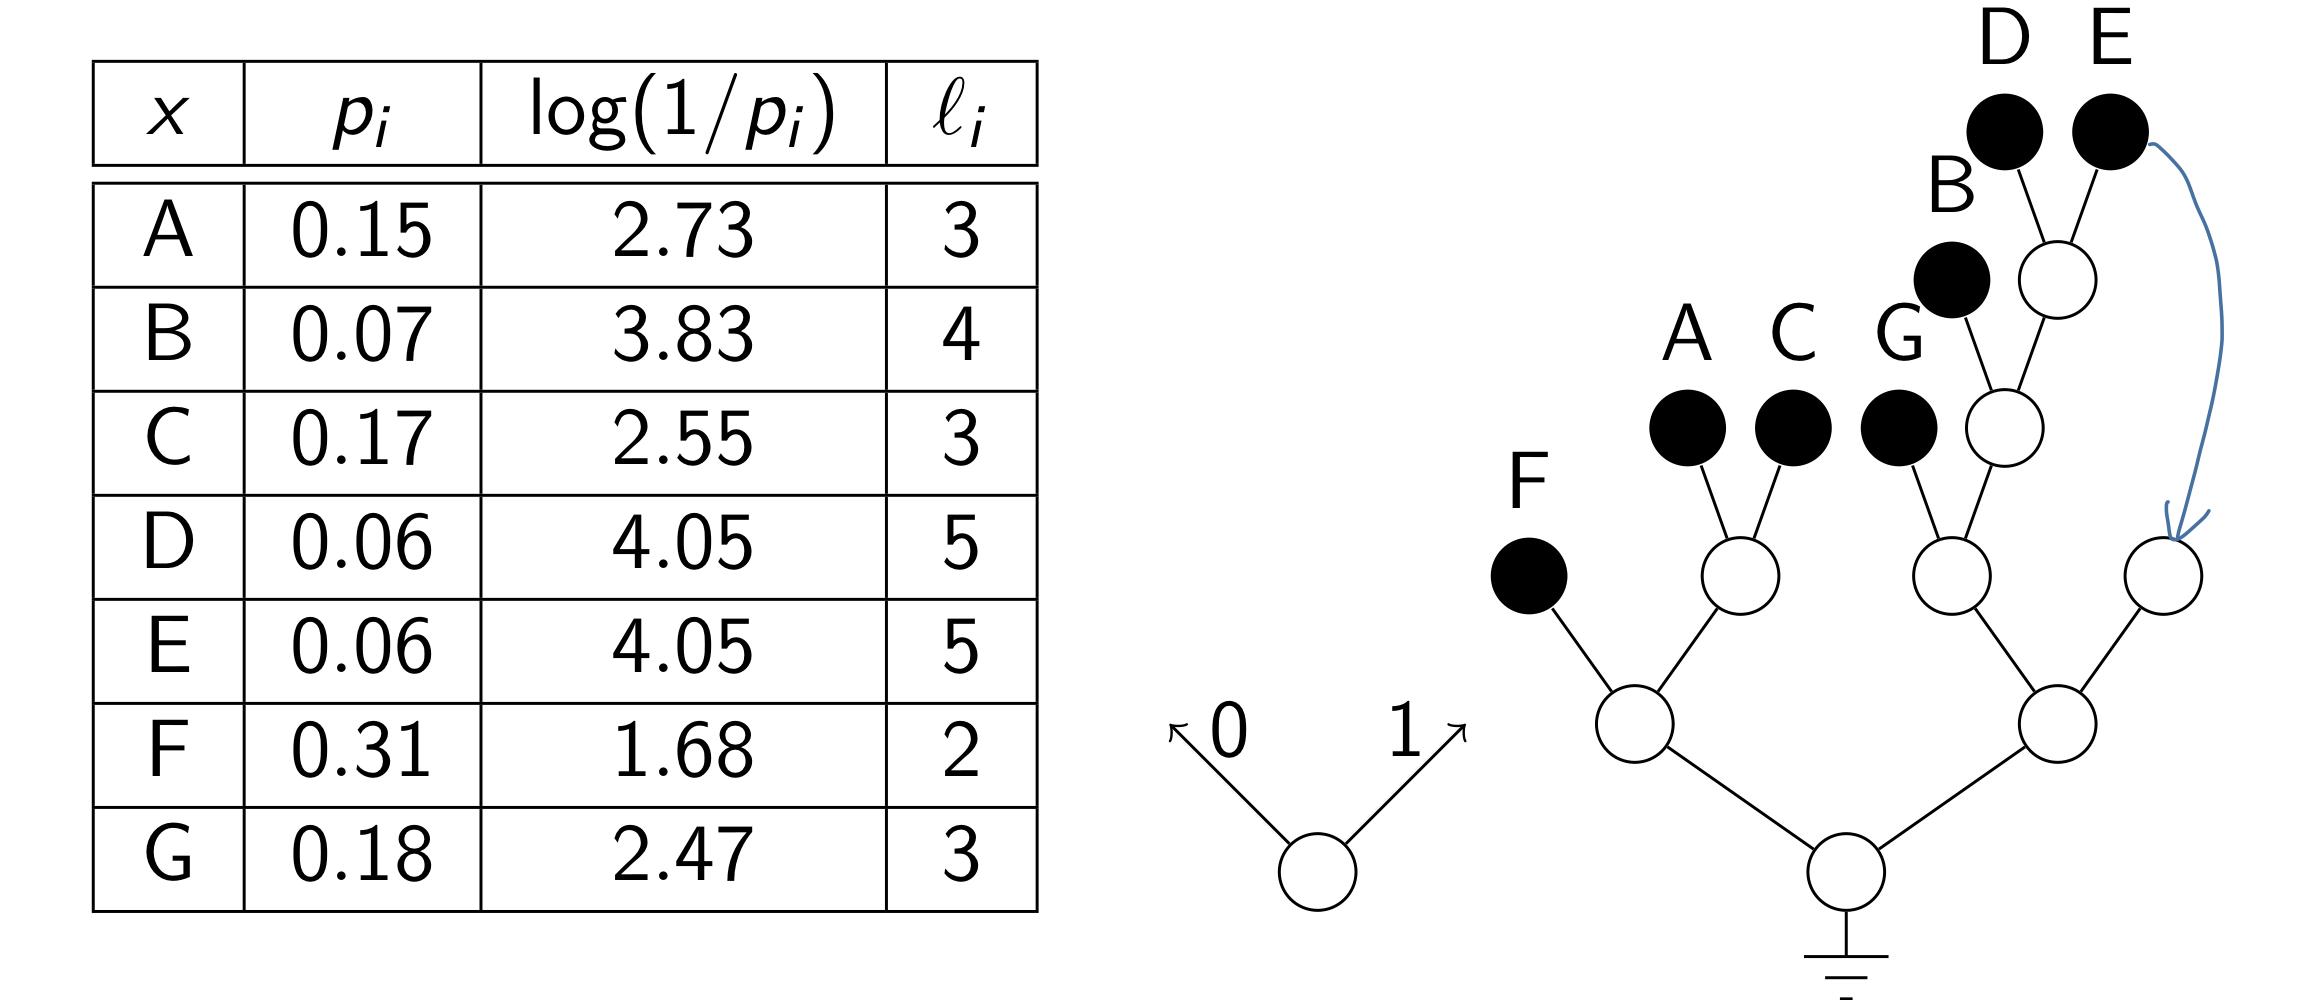
\includegraphics[width=0.8\linewidth ]{Shannon.png}
  \label{fig:1}
\end{figure}
\item Clearly, we can do better by pushing B/D/E to the length two
\end{itemize}

\subsection{Properties of Optimal prefix-free code}
\begin{enumerate}
\item The lengths are ordered inversely with the probabilities, if $p_j > p_k,$ then $\mathit{l}_j \le \mathit{l}_k$  
\item The two last probable symbols have the same length and are on neighboring leaves in the binary tree (i.e. they differ only in the last digit).
\end{enumerate}

\subsection{Huffman Coding}
\begin{itemize}
\item An algorithm gives an optimal prefix-free code for a given set of probabilities.
\begin{enumerate}
\item Take the two least probable symbols in the alphabet. these two symbols will be given the longest codewords, which will have equal length, and differ only in the last digit
\item Combine these two symbols into a single symbol, and repeat.
\end{enumerate}

\item A source produces symbols from the set \{A,B,C,D,E,F\} with probabilities \{0.05,0.1,0.15,0.2,0.2,0.3\}
\begin{enumerate}
\item List these symbols in increasing order of their probabilities.
\begin{figure}[h]
\begin{subfigure}[h]{0.3\linewidth}
  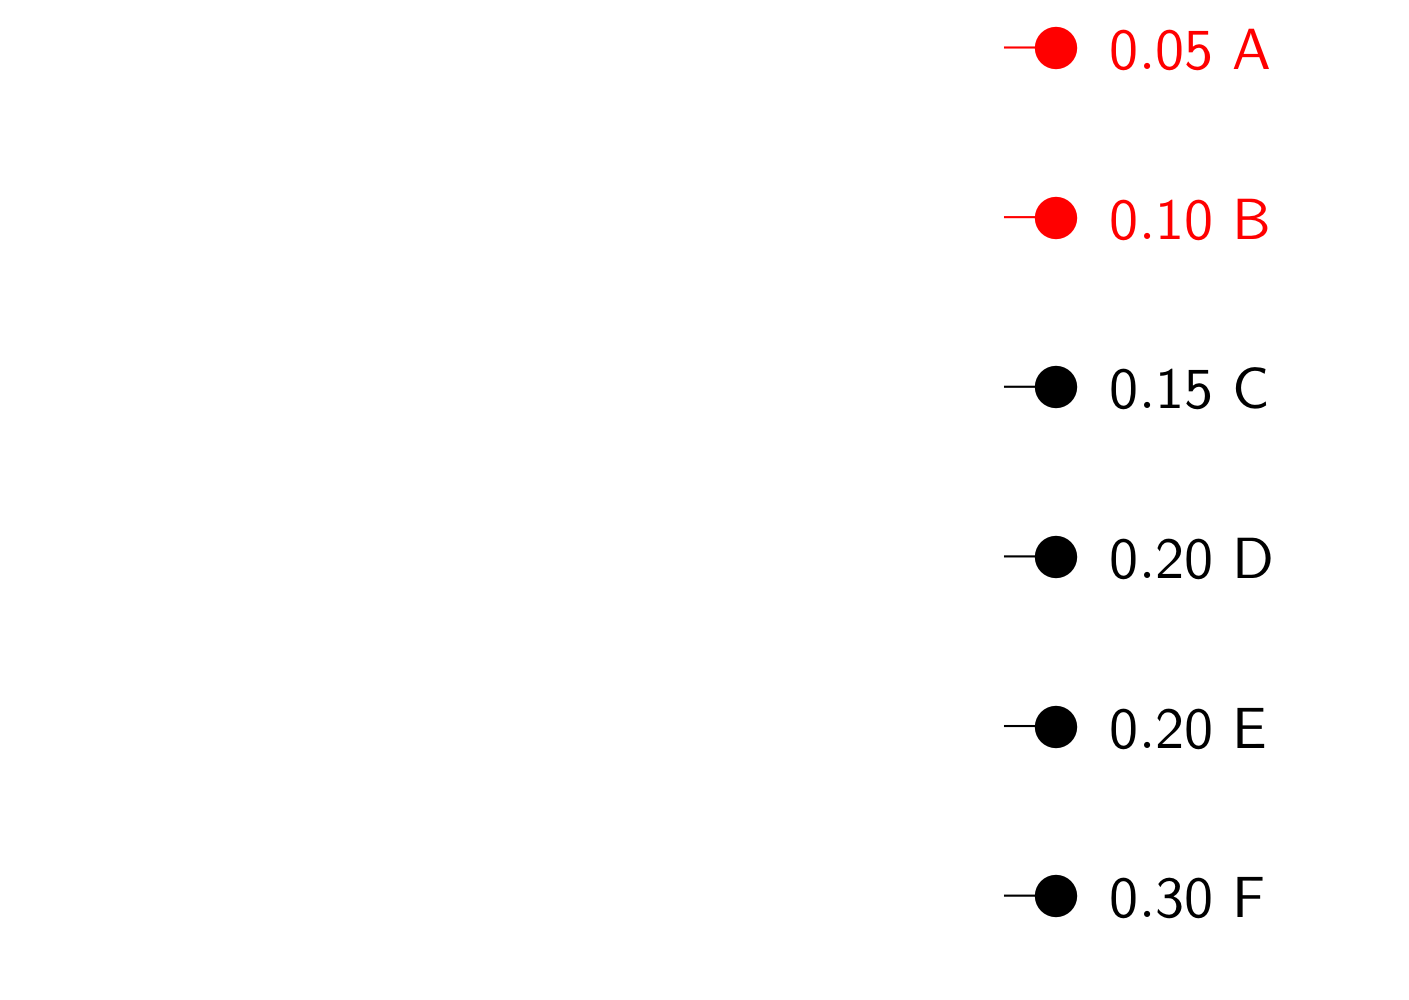
\includegraphics[width=\linewidth]{Huff1.png}
  \caption{Step 1}
\end{subfigure}
\begin{subfigure}[h]{0.3\linewidth}
  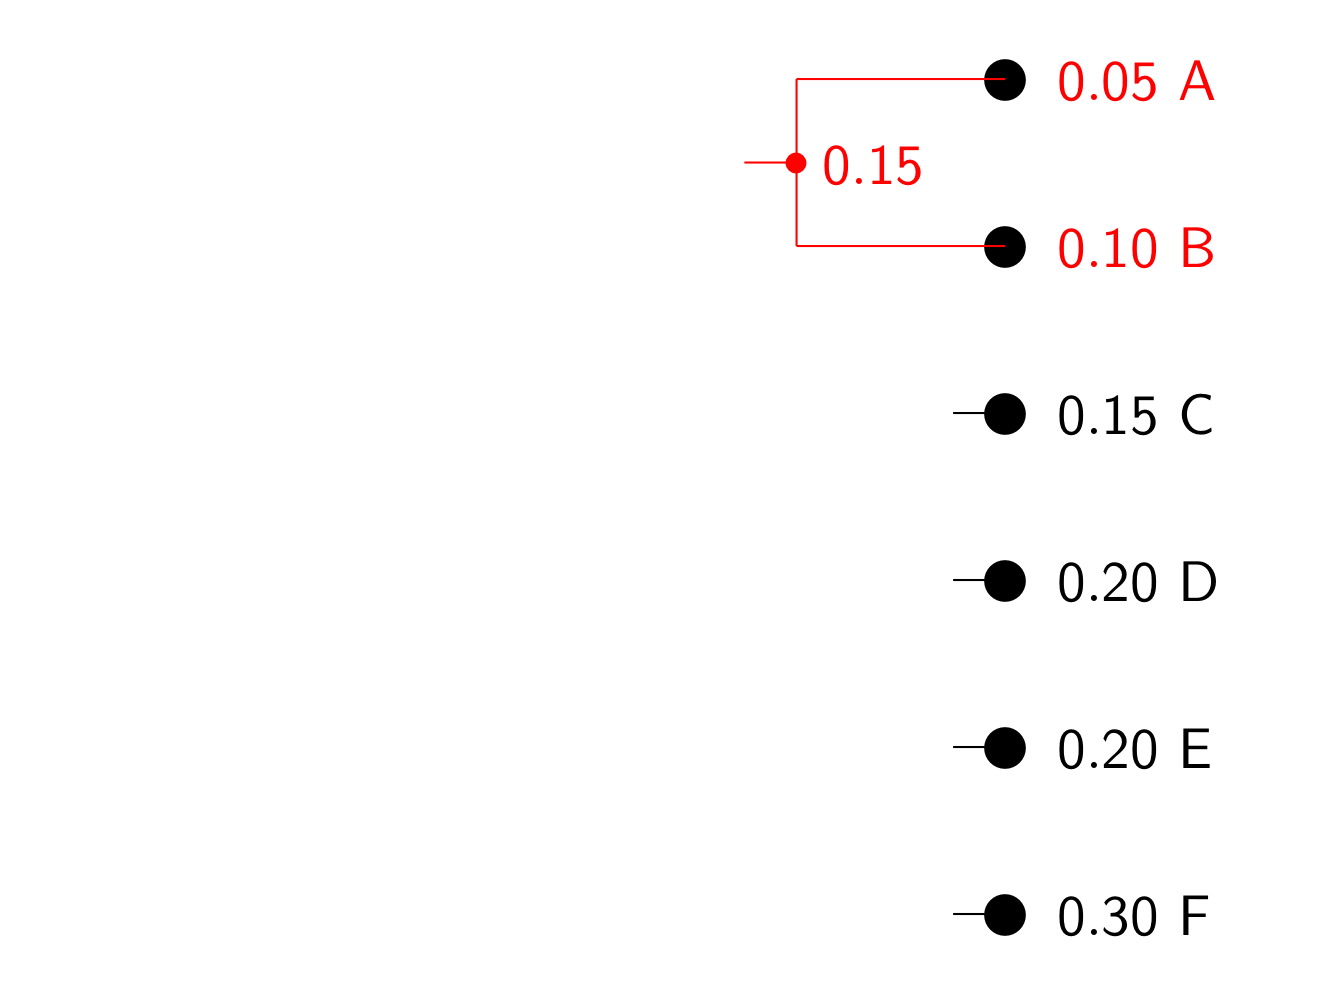
\includegraphics[width=\linewidth] {Huff2.png}
  \caption{Step 2}
\end{subfigure}
\begin{subfigure}[h]{0.3\linewidth}
  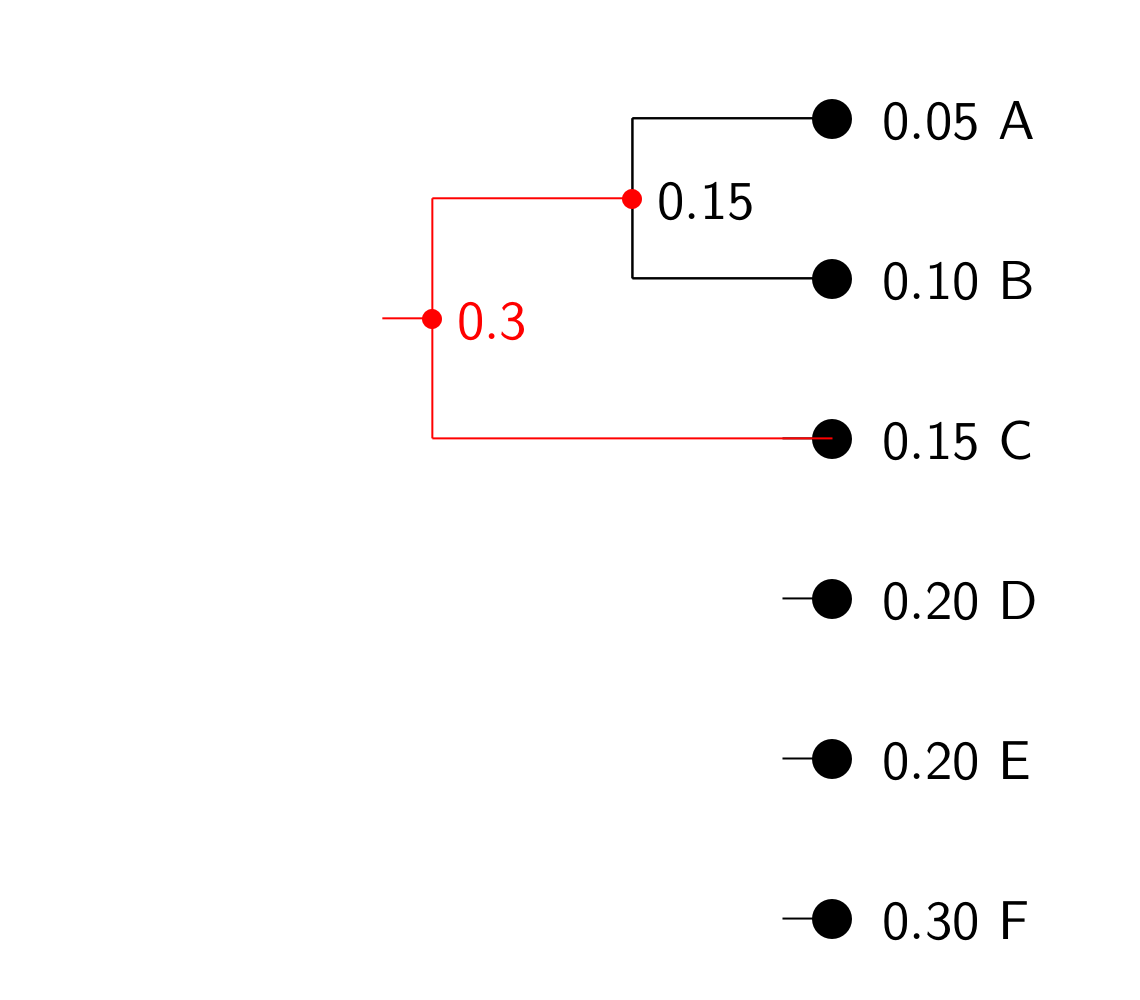
\includegraphics[width=\linewidth]{Huff3.png}
  \caption{Step 3}
\end{subfigure}
\end{figure}
\item Combine the two simple with the smallest probabilities, and form a "super-symbol" with the sum of their probabilities.

\item We now have five symbols with probabilities \{0.15,0.15,0.2,0.2,0.3\}. Again combine the two symbols with the smallest probabilities...

\item Among the four remaining symbols, D,E have the smallest probabilities, so combine
\begin{figure}[h]
\begin{subfigure}[h]{0.3\linewidth}
  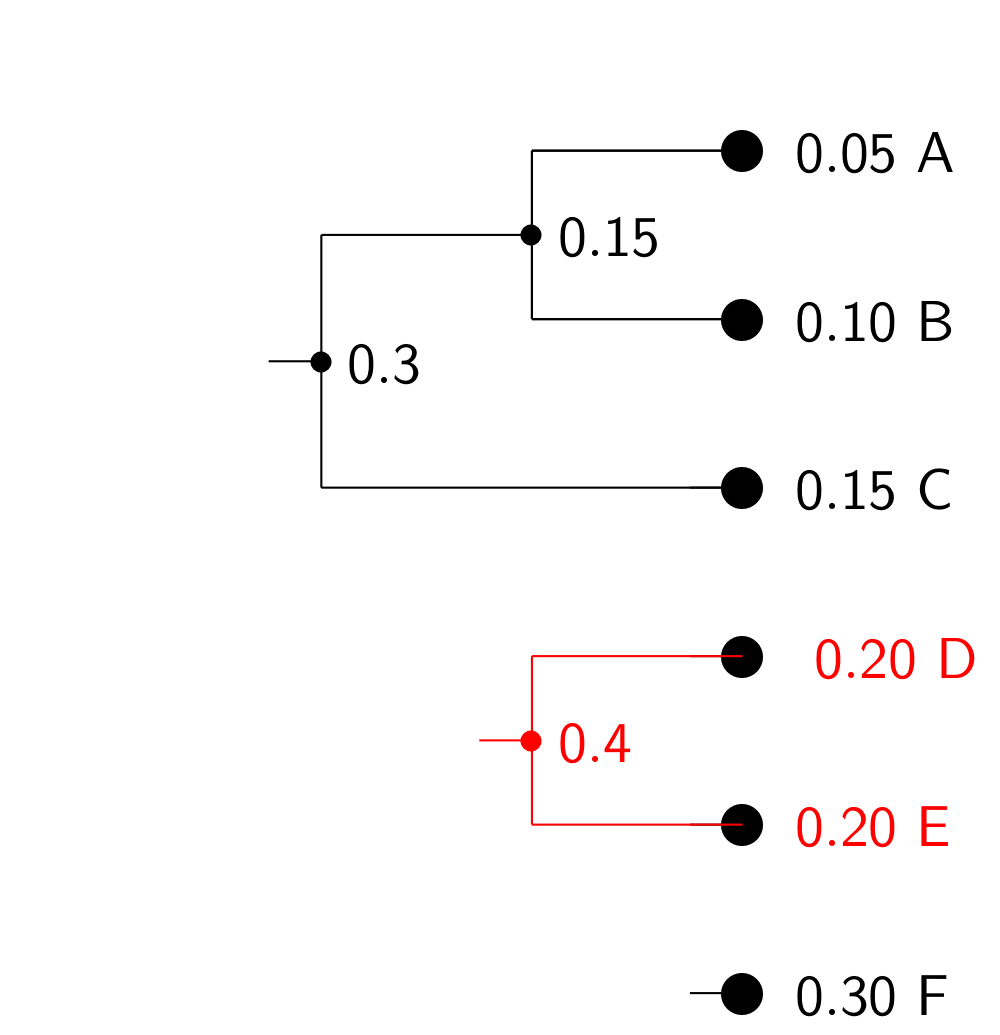
\includegraphics[width=\linewidth ]{Huff4.png}
  \caption{Step 4}
\end{subfigure}
\begin{subfigure}[h]{0.3\linewidth}
  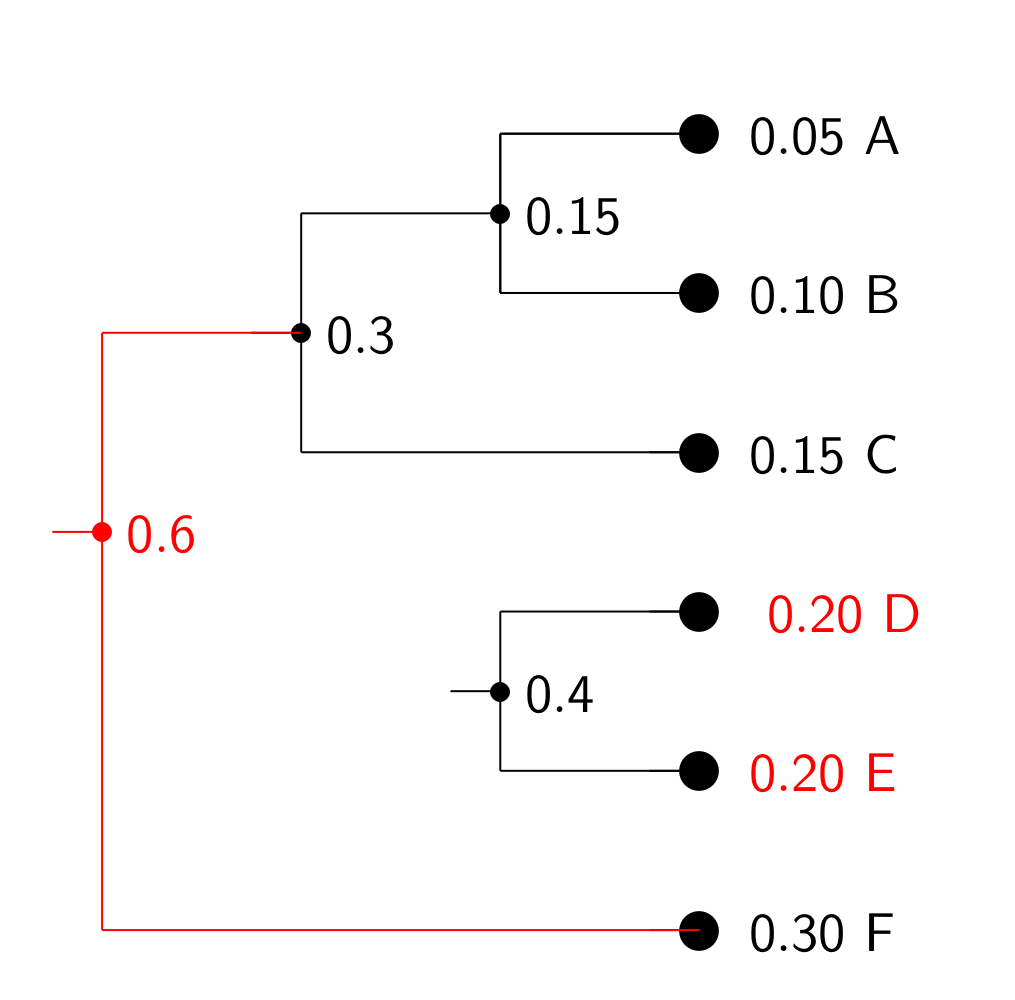
\includegraphics[width=\linewidth ]{Huff5.png}
  \caption{Step 5}
\end{subfigure}
\begin{subfigure}[h]{0.3\linewidth}
  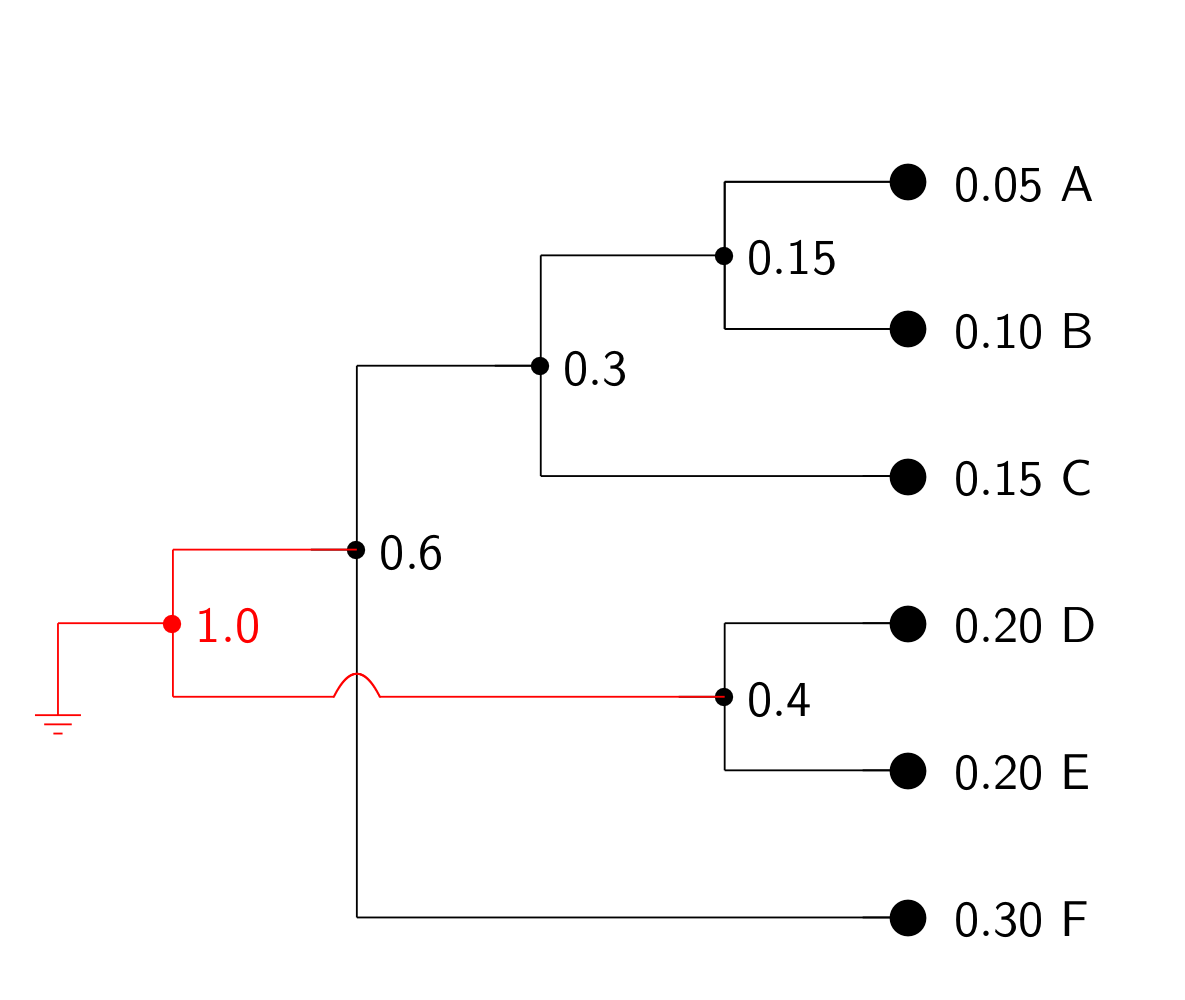
\includegraphics[width=\linewidth ]{Huff6.png}
  \caption{Step 6}
\end{subfigure}
\end{figure}
\item Among the three remaining symbols, the smallest probabilities are {0.3,0.3}, so combine them...

\item Finally, combine the remaining two symbols 

\item The symbols are the leaves of a tree. The final step is to assign the codewords to the symbols using the tree.
\begin{figure}[h]
  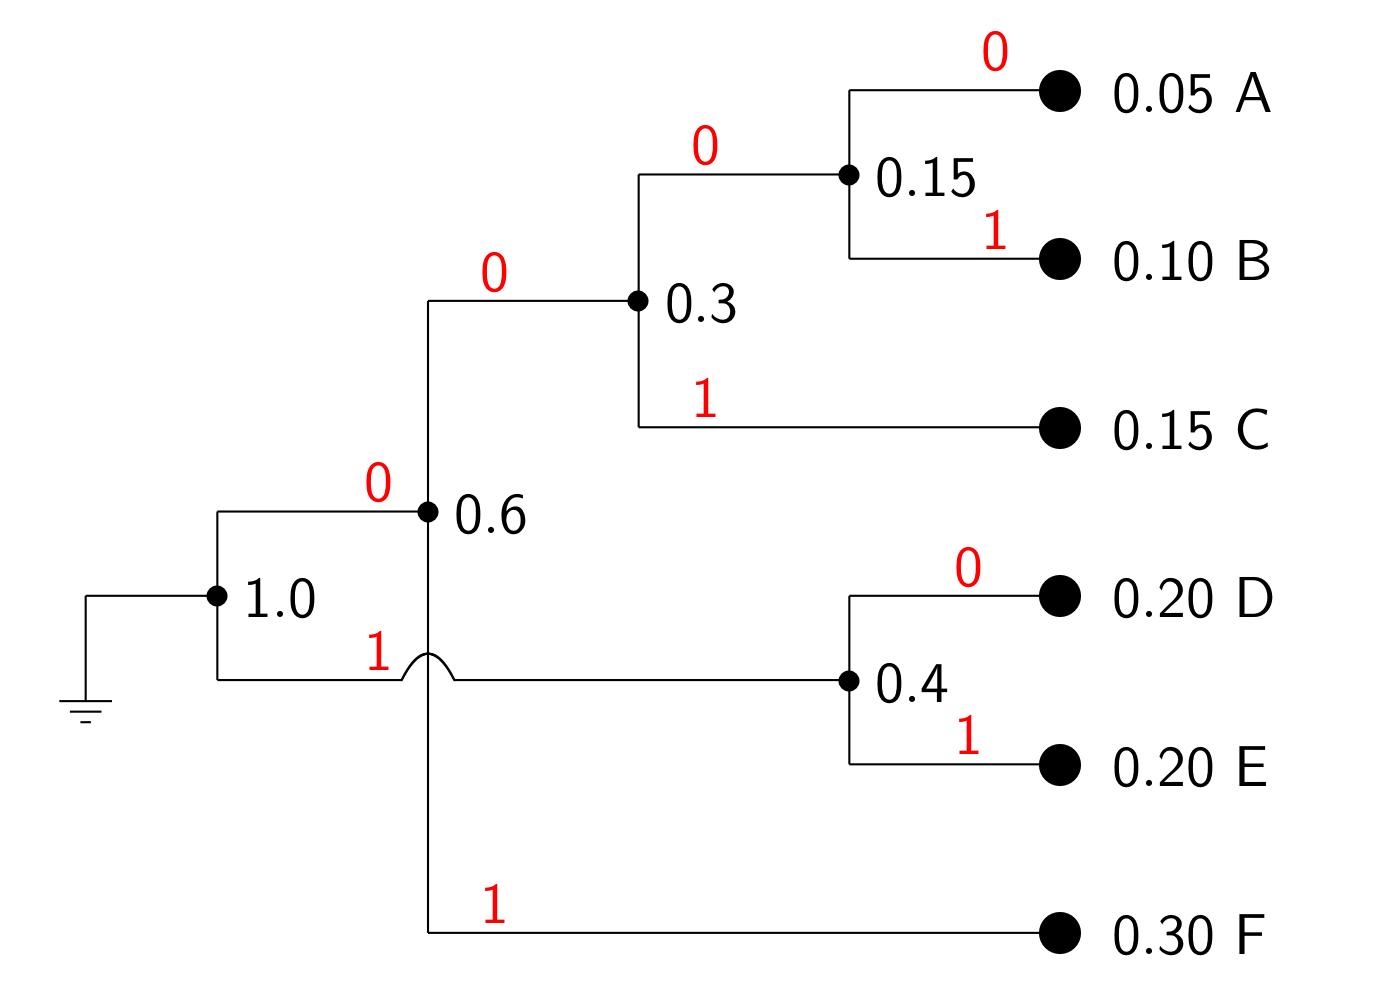
\includegraphics[width=0.3\linewidth ]{Huff7.png}
  \caption{Assign codes}
\end{figure}
\end{enumerate}
The Huffman code is:
$$F \rightarrow 01, E \rightarrow 11, D \rightarrow 10, C \rightarrow 001, B \rightarrow 0001, A \rightarrow 0000$$

\item Properties of the Huffman Code 
\begin{enumerate}
\item For a source with alphabet of size m, the Huffman algorithm requires $m-1$ steps of combining the two smallest probabilities at each stage.

\item The Huffman code for a given source may not be unique: Swapping 0/1, also 3 same prob can take any two. However, the expected code length should be the same.


\end{enumerate}
\item Optimality of Huffman coding: For a given set of probabilities, there is no prefix-free code that has smaller expected length than the Huffman code.

\item Huffman codes are optimal for coding a single random variable X, and have expected code length that is less than $H(X) + 1$ But they have some weaknesses:
\begin{itemize}
\item To reduce this overhead of up to 1 bit/symbol, we could design a Huffman code for blocks of k symbols. This would give us an overhead of 1 bit/k symbols, or 1/k bits/symbols.
\item But this comes with the expense of increased complexity. For blocks of k symbols, the binary tree is much larger.
\item These defects are addressed by Arithmetic coding, a scalable algorithm whose expected code length is very close to the source entropy for large sequences. It can also easily deal with non-iid source like text.
\end{itemize}

\end{itemize}

\subsection{Interval Coding}
\begin{itemize}
\item Key idea: Each symbol can be represented as an interval inside $[0,1]$ with length of the interval equal to the symbol probability. 

A source with m symbols with probabilities $\{ p_1,...,p_m\}$ is represented using m intervals 

\[
[0,p_1), [p_1, p_1+p_2),...,[\sum_{i=1}^{m-1}p_i, \sum_{i=1}^{m-1}p_i + p_m).
\]
\item Example: To represent interval $[0.17,0.43)$ convert the end-points to binary and find a binary interval lies completely inside this interval. say $[010,011]$ is the interval of $[0.25,0.375]$ We choose \textbf{010} as the codeword for $[0.17,0.43)$.

\item In general, the binary codeword for a symbol with probability p represented by the interval $[a,a+p)$ can be obtained as follows:
\begin{enumerate}
\item Find the largest \textit{dyadic interval} of the form $[\frac{j}{2^{\mathit{l}}}, \frac{j+1}{2^{\mathit{l}}})$ that lies within $[a,a+p)$
\item Take the binary representation of the lower end-point of the dyadic interval as the codeword.
\end{enumerate}
\item Code length: With $\mathit{l}$ code bits, the dyadic intervals have length $2^\mathit{l}$. The dyadic interval has to be contained within an interval of length p. Hence 
\[
2^\mathit{l} \le p \rightarrow \lceil \log_2(1/p) \rceil \le \mathit{l}
\]
But sometimes we'll need $\mathit{l} =\lceil \log_2(1/p) \rceil +1 $ \\
The expected code length can therefore be bounded as 
\[
L = \sum_i p_i\mathit{l}_i \le \sum_i p_i (\lceil \log_2(1/p_i) \rceil +1) < H(X) + 2
\]
\item Performance: In terms of expected code length, the analysis above shows that interval codes are in general not as good as Huffman codes or even Shannon-Fano codes. But interval coding is the basis for arithmetic coding, which is a powerful technique for long source sequences.

\end{itemize}
\subsection{Arithmetic Coding}
\begin{itemize}

\item Explain with an example. Consider a source producing symbols $X_1,X_2,...,X_n$ which are i.i.d., with each $X_i$ taking values in $\{a,b,c\}$ with probabilities $\{0.2,0.45,0.35\}$
\item Key ideas:
\begin{itemize}
\item Each length n string $(x_1,...,x_n)$ is represented by a disjoint interval with length equal to the probability of the string. 
\begin{itemize}
\item E.g. for $n=2$, $X_1=b,X_2=c$ corresponds to the probability of length $0.45 * 0.35=0.1575$ and $X_1=b,X_2=a$ of length $0.45 * 0.2=0.09$.
\end{itemize}
\item The interval for $(X_1=x,X_2=y)$ is a sub interval of the interval for $X_1=x$ 
\begin{itemize}
\item E.g. $X_1 = b$ is the interval $[0.2,0.65)$ and $(X_1 = b, X_2=c)$ is the subinterval of length $0.1575$ within  $[0.2,0.65)$ To calculate, we rewrite the interval as $\{0,0.2,0.65,0.1\}$ as the order of a,b,c.
\item The subinterval becomes $0.2 + (0.65-0.2) * 0.65 \rightarrow 0.2 + (0.65-0.2) * 1$ That is $[0.4925,0.65)$ Also we can verify that $0.65 - 0.4925 = 0.1575$
\end{itemize}  
\item Similarly, for any symbols $x,y,z$, $P(X_1=x,X_2=y,X_3=z)$ is a sub interval of $P(X_1=x,X_2=y),$ and so on.
\end{itemize}
\item Decoding: Using binary codeword to sequentially zoom in to the interval, decoding symbols as you go along.
\item Expected code length:\\
Arithmetic coding can be performed in any sequence of length n, so that any sequence $x_1,...,x_n$ can be represented by an interval of length $p(x_1,...,x_n)$, which gives a binary codeword of length at most $\lceil \log_2\frac{1}{p(x_1,...,x_n)} \rceil + 1$. \\
Therefore the expected code length for length n sequences is bounded as:
\[
L_n = \sum_{X_n} p_{x_n}\mathit{l}_{x_n} \le \sum_{x_n} p_{x_n} (\log_2\left(1/p(x_1,...,x_n)\right)+2) = H(X^n) + 2
\]
Therefore the expected code length per symbol is 
\[
\frac{L_n}{n} < \frac{H(X^n)}{n} + \frac{2}{n} = H(X) + \frac{2}{n},
\]
Where the last equality hold for $iid ~ P_X$
\end{itemize}
\subsection{Arithmetic coding for non-iid sources}
\begin{itemize}
\item Consider a source that produces symbols in alphabet $\{ a_1,...,a_m\}$ with a known distribution 
\[
P(x_1)p(x_2|x_1)...P(x_n|x_1,...,x_{n-1})
\]
The arithmetic coding algorithm can be easily extended to such sources. As before, consider the source with alphabet $\{a,b,c\}$ with probabilities $\{0.2,0.45,0.35\}$. \\
Suppose that three conditional distributions $P(X_2|X_1=a)$, $P(X_2|X_1=b)$, $P(X_2|X_1=c)$ and say
\[
P(X_2=a|X_1=b)=0.5 , P(X_2=b|X_1=b)=0.3, P(X_2=c|X_1=b)=0.2
\]
We do the same thing as before, just change the probability using the conditional probability accordingly.
\item Coding Algorithm:
\begin{itemize}
\item Let source alphabet $\mathcal{A}$ be $\{ a_1,...,a_m\}$
\item We are given a source sequence $x_1,x_2,...,x_n$ where each $x_i \in \mathcal{A}$
\item Both encoder and decoder know the conditional distributions $P_{X_1}, P_{X_2|X_1},...,P_{X_n|X_1,...,X_{n-1}}.$
\item The encoding algorithm computes the interval using the following lower and upper cumulative probabilities.
For $i=1,...m$ and for $k-1,...,n$ we define 
\[
L_k(a_i|x_1,...,x_{k-1}) = \sum_{i^{\prime}}^{i-1}  P(X_k=a_{i^{\prime}} | X_1=x_1,...,X_{k-1}=x_{k-1}) 
\]

\[
U_k(a_i|x_1,...,x_{k-1}) = \sum_{i^{\prime}}^{i}  P(X_k=a_{i^{\prime}} | X_1=x_1,...,X_{k-1}=x_{k-1})
\]
\end{itemize}
\item Finite precision issues:
The arithmetic encoding algorithm above assumes an infinite precision computer:
\begin{itemize}
\item As n grows, the length of the interval corresponding to a sequence $(x_1,...,x_n)$ shrinks
\item Hence the number of digits needed to accurately store the values lo and hi grows with n.
\end{itemize}
\end{itemize}
Summary:
\begin{enumerate}
\item Arithmetic coding can achieve compression very close to the source entropy, with complexity scaling linearly with the length of the sequence.
\item It does require you to know the conditional distribution. But this approach fits well with machine learning techniques that can mine huge quantities of text/speech/video data to build good probabilistic models.
\item Note that the assumed distribution of the source doesn't need to be true one, it only needs to be the same at both encoder and decoder.
\item Arithmetic coding works even when you generate the source conditional distribution on the fly, based on what has been observed so far. Given the generating rule, the decoder will also generate required conditional distributions as it reconstructs the sequence.
\end{enumerate}

\section{Relative Entropy Mutual Information}
\subsection{Relative Entropy}
\subsubsection{Define}
The \textbf{\textit{Relative Entropy}} or the \textit{Kullback-Leibler(KL)} divergence between two pmfs P and Q is:

\[
D(P||Q) = \sum_{x \in \rchi}P(x)\log\frac{P(x)}{Q(x)}
\]

\begin{itemize}
\item P and Q are defined on the same alphabet $\rchi$
\item Measure of distance between distributions  P and Q
\item Not a true distance. For example:  $D(P||Q) \not = D(Q||P)$
\item if $P=Q$ Then $D(P||Q) = 0$
\item Example: If $P= Bern(p) $ and $Q= Bern(q)$ for $p,q \in [0,,1],$
\[
D(P||Q) = p\log\frac{p}{q} + (1-p)\log\frac{1-p}{1-q}
\] 
\item Relative Entropy is always non-negative:
\[
D(P||Q) \ge 0 \textrm{With equality if and only if } P=Q
\]
\textit{Proof:} Using $\log_2a = \frac{\ln a}{\ln 2}$
\begin{align*}
-D(P||Q) & = \frac{1}{\ln 2} \sum_{x \in \rchi} P(x) \ln\frac{Q(x)}{P(x)} \\
& \le  \frac{1}{\ln 2} \sum_{x \in \rchi} P(x)\left( frac{Q(x)}{P(x)}\right) 
& = \frac{1}{\ln 2} (1-1) = 0
\end{align*}
Again, we use our favorite inequality $\ln x \le (x-1)$ with equality $iff$  x=1
\item We look at applications in \textcolor{blue1}{compression} and \textcolor{blue1}{hypothesis testing}.
\end{itemize}
\subsubsection{Redundancy in Source Coding}
Often the \textcolor{blue1}{True distribution} of the source is unknown, and we have to work with estimated source distribution for compression.
\begin{itemize}
\item Suppose \textcolor{blue}{true pmf} of a rv is $P = \{ p_1,...,p_m\}$, \textcolor{orange}{estimated pmf} is $\hat{P} = \{ \hat{p}_1,...,\hat{p}_m\}$
\item $\hat{P}$ is used to design a compression code whose code length $\mathit{l}_i$ satisfy
\[
\textcolor{red}{ \mathit{l}_i = \log(1/\hat{p}_i) }\qquad \textrm{for } i=1,...,m.
\]
The code is optimal for the distribution $\hat{p}$
\item How far are we from the optimal of the \textcolor{blue1}{true distribution}?
The Average code Length:
\begin{align*}
L = \sum_ip_i\mathit{l}_i & = \sum_{i}p_i \log \frac{1}{\hat{p}_i} \\
& = \sum_{i}p_i \log\frac{p_i}{p_i\hat{p}_i} \\
& = \sum_{i}p_i \log\frac{1}{p_i} + \sum_{i}p_i \log\frac{p_i}{\hat{p}_i} \\
& = H(P) + D(P||\hat{p}_i) \quad \textrm{bits/symbol}
\end{align*}
\item Therefore  $D(P||\hat{p}_i)$ is the \textcolor{red}{Price} you pay in bits/symbol --Redundancy-- for designing the code with estimated distribution rather than true distribution.

\item Example:  

\end{itemize}

\subsubsection{Hypothesis Testing}

\subsection{Mutual Information}


\subsection{Conditional Mutual Information and chain Rule}


\section{Discrete Channels and Channel Capacity}

\subsection{Communication Channel}

\subsection{Binary Channel}


\subsection{Channel Capacity}


\section{Channel Coding Theorem}

\section{Data Processing, Fano's Inequality}
\subsection{Data Processing and Mutual Information}
\subsection{Fano's Inequality}

\subsection{In term of Channel Coding}

\subsection{Channel Coding Converse}

\section{Information theory with continuous RVs}

\subsection{The Additive White Gaussian Noise(AWGN) Channel}

\subsection{Information Theory for Continuous Alphabets}

\section{Binary Linear Block Codes}




\section{Low Density Parity Check(LDPC) Codes for the Binary Erasure Channel}




\end{document}
